%FILL IN THE RIGHT INFO.
%\lecture{**LECTURE-NUMBER**}{**DATE**}
\unchapter{Lecture 4}
\lecture{4}{September 15}
\setcounter{section}{0}
\setcounter{theorem}{0}

% **** YOUR NOTES GO HERE:


\section{Integrals over Closed Curves}

\subsection{Goursat's Theorem}
We start by presenting the following theorem:

\isubsection{THM: Goursat's Theorem}

\begin{theorem}
Open $\Omega \subset \mathbb{C}$, $f: \Omega \rightarrow \mathbb{C}$ holomorphic. Let $T\subset \Omega$ be a (solid) triangle (this is piecewise smooth). Then:

\begin{align*}
    \int_{\partial T} f(z)  \dif z =0\\
\end{align*}

\end{theorem}


\begin{proof}
Consider a triangle T in an open set $\Omega$.




\begin{center}
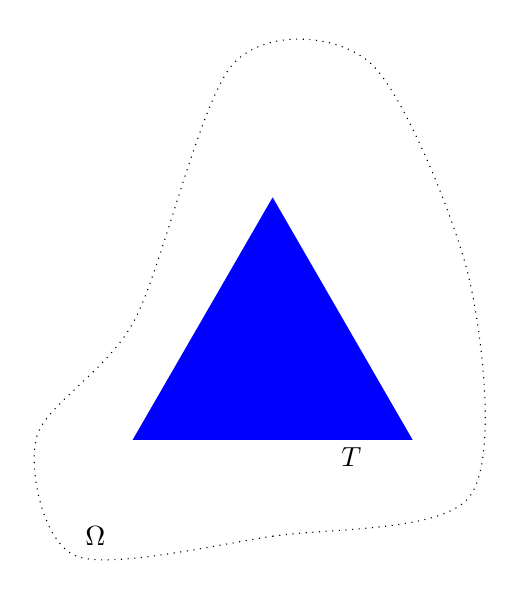
\begin{tikzpicture}
    \draw[shift={(-2.5,-2.5)},rotate=0][dotted][scale =2.5] plot [smooth cycle] coordinates {(0,0) (1,0.1) (2,0.3) (2,1.4) (1.5,2.5) (0.8,2.5) (0.3,1.2) (-0.2,0.6) };
    \draw (-2.25,-2.25) node {$\Omega$};
    
    \draw[fill=blue][scale=2] [blue,line width=1.5pt] (90:1) -- (330:1) -- (210:1) -- cycle;
    
    \draw (1,-1.25) node {$T$};
\end{tikzpicture}    
\end{center}

Subdivide T as follows: pick the midpoints of the sides, and form 4 smaller triangles by joining these points, then label these triangles $T^1,T^2,T^3,T^4$ such that $T=T^1 \cup T^2 \cup T^3 \cup T^4$:

\begin{center}
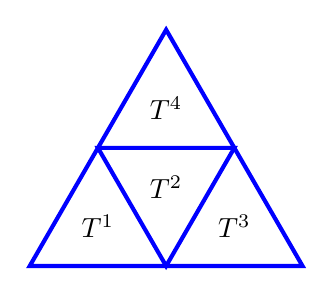
\begin{tikzpicture}
    \draw[scale=2] [blue,line width=1.5pt] (90:1) -- (330:1) -- (210:1) -- cycle;
    \draw[rotate=180][blue,line width=1.5pt] (90:1) -- (330:1) -- (210:1) -- cycle;
    \draw (0,0) node {$T^2$};
    \draw (90:1) node {$T^4$};
    \draw (90+120:1) node {$T^1$};
    \draw (90+240:1) node {$T^3$};
\end{tikzpicture}    
\end{center}

We use the positive orientation (CCW) for boundaries of triangles.


\begin{center}
%absolute cancer solution and it embarrasses me but idk how else to do this
%after some mulling maybe try applying the postaction to 1/6, 3,6 5,6 instead of 1/2 ??
\begin{tikzpicture}[very thick,decoration={
    markings,
    mark=at position 0.5 with {\arrow{<}}}
    ]
\draw[rotate =180][postaction={decorate}] [blue,line width=1.5pt] (90:1) -- (330:1) -- (210:1) -- cycle;
    \draw[rotate =60][postaction={decorate}] [blue,line width=1.5pt] (90:1) -- (330:1) -- (210:1) -- cycle;
    \draw[rotate =300][postaction={decorate}] [blue,line width=1.5pt] (90:1) -- (330:1) -- (210:1) -- cycle;
    
    \draw[shift=(90:1.5)][postaction={decorate}] [blue,line width=1.5pt] (90:1) -- (330:1) -- (210:1) -- cycle;
    \draw[rotate=120, shift=(90:1.5)][postaction={decorate}] [blue,line width=1.5pt] (90:1) -- (330:1) -- (210:1) -- cycle;
    \draw[rotate=240, shift=(90:1.5)][postaction={decorate}] [blue,line width=1.5pt] (90:1) -- (330:1) -- (210:1) -- cycle;
    
    
    \draw[shift=(210:1.5)][postaction={decorate}] [blue,line width=1.5pt] (90:1) -- (330:1) -- (210:1) -- cycle;
    \draw[rotate= 120,shift=(210:1.5)][postaction={decorate}] [blue,line width=1.5pt] (90:1) -- (330:1) -- (210:1) -- cycle;
    \draw[rotate=240,shift=(210:1.5)][postaction={decorate}] [blue,line width=1.5pt] (90:1) -- (330:1) -- (210:1) -- cycle;
    
    
    
    \draw[shift=(330:1.5)][postaction={decorate}] [blue,line width=1.5pt] (90:1) -- (330:1) -- (210:1) -- cycle;
    \draw[rotate=120, shift=(330:1.5)][postaction={decorate}] [blue,line width=1.5pt] (90:1) -- (330:1) -- (210:1) -- cycle;
    \draw[rotate= 240,shift=(330:1.5)][postaction={decorate}] [blue,line width=1.5pt] (90:1) -- (330:1) -- (210:1) -- cycle;
    
    
    \draw (0,0) node {$T^2$};
    \draw (90:1.5) node {$T^4$};
    \draw (90+120:1.5) node {$T^1$};
    \draw (90+240:1.5) node {$T^3$};
    
    
\end{tikzpicture}
\end{center}

Let $I=\int_{\partial T} f(z)  \dif z$. Observe that (since integrating over a curve backwards cancels with integrating over a curve forwards):

\begin{align*}
    I&=\int_{\partial T} f(z)  \dif z\\
    &=\sum_{n=1}^{4}\int_{\partial T^n} f(z)  \dif z
\end{align*}

Let $T_1^i = T^i$, $i=1,2,3,4$: 

\begin{center}
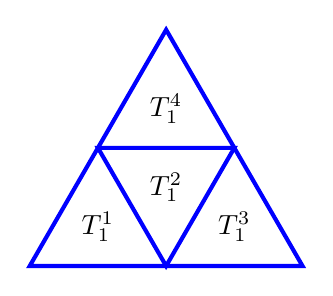
\begin{tikzpicture}
    \draw[scale=2] [blue,line width=1.5pt] (90:1) -- (330:1) -- (210:1) -- cycle;
    \draw[rotate=180][blue,line width=1.5pt] (90:1) -- (330:1) -- (210:1) -- cycle;
    \draw (0,0) node {$T^2_1$};
    \draw (90:1) node {$T^4_1$};
    \draw (90+120:1) node {$T^1_1$};
    \draw (90+240:1) node {$T^3_1$};
\end{tikzpicture}    
\end{center}

\begin{align*}
I &= \sum_{n=1}^{4}\int_{\partial T^n_i} f(z)  \dif z\\
\abs{I} &= \abs{\sum_{n=1}^{4}\int_{\partial T^n_i} f(z)  \dif z}\\
&\leq \sum_{n=1}^{4} \underbrace{\abs{\int_{\partial T^n_i} f(z)  \dif z}}_{\text{one of these is } \geq \frac{\abs{I}}{4} }\\
\end{align*}

WLOG we say that this is the first triangle:

\begin{align*}
    \abs{\int_{\partial T_1^1} f(z)  \dif z} \geq \frac{\abs{I}}{4}
\end{align*}

We then subdivide $T_1^1$ into 4 more triangles $T_2^1,T_2^2,T_2^3,T_2^4$:


\begin{center}
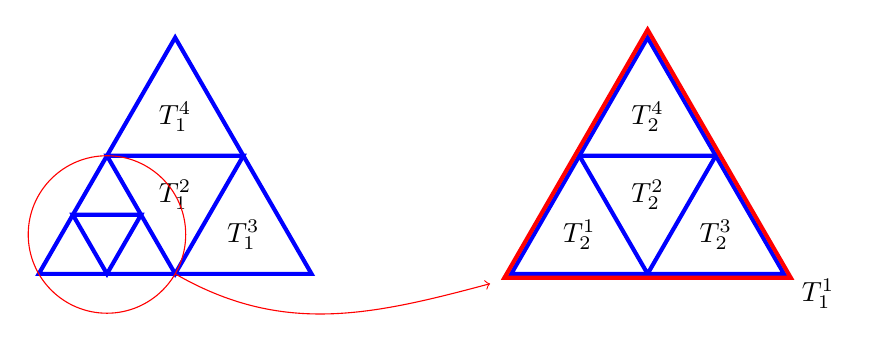
\begin{tikzpicture}

    \draw[scale=2] [blue,line width=1.5pt] (90:1) -- (330:1) -- (210:1) -- cycle;
    \draw[rotate=180][blue,line width=1.5pt] (90:1) -- (330:1) -- (210:1) -- cycle;
    \draw[scale=0.5][rotate=180, shift = (90+120:-2)][blue,line width=1.5pt] (90:1) -- (330:1) -- (210:1) -- cycle;
    \draw[shift=(0:0)] (0,0) node {$T^2_1$};
    \draw[shift=(0:0)] (90:1) node {$T^4_1$};
    \draw[shift=(0:0)] (90+240:1) node {$T^3_1$};
    \draw [color=red] (90+120: 1) circle (1);
    \draw[color = red][->] (90+120: 1)+(90+240:1) to [out=-30,in=195] (4,-1.125);


    \draw[shift=(0:6)][scale=2] [blue,line width=1.5pt] (90:1) -- (330:1) -- (210:1) -- cycle;
    \draw[shift=(0:6)][rotate=180][blue,line width=1.5pt] (90:1) -- (330:1) -- (210:1) -- cycle;
    \draw[shift=(0:6)] (0,0) node {$T^2_2$};
    \draw[shift=(0:6)] (90:1) node {$T^4_2$};
    \draw[shift=(0:6)] (90+120:1) node {$T^1_2$};
    \draw[shift=(0:6)] (90+240:1) node {$T^3_2$};
    \draw[shift=(0:6)] (90+240:2.5) node {$T^1_1$};
    \draw[shift=(0:6)][scale=2] [red,line width=1.5pt] (90:1.05) -- (330:1.05) -- (210:1.05) -- cycle;
\end{tikzpicture}    
\end{center}

We then repeat the argument just performed on the sub-triangles as well. This yields:

\begin{align*}
    \abs{\int_{\partial T_2^1} f(z)  \dif z} &\geq \frac{1}{4} \abs{\int_{\partial T_1^1} f(z)  \dif z} \geq \frac{\abs{I}}{4^2}
\end{align*}


Repeating this we get:

\begin{align}
    \abs{\int_{\partial T_k^1}f(z)  \dif z}  &\geq \frac{\abs{I}}{4^n}
\end{align}
    for the nested triangles $T \supset T_1^1 \supset T_2^1 \supset \cdots \supset T_k^1 \supset \cdots$.\\\\
We also know that:

\begin{align*}
    \text{with } diam(K) &= \sup\{ \, \abs{z-w} : z,w\in K \}\\
    diam(T_k^1) &= \frac{diam(T)}{2^k} \xrightarrow[]{\text{as } k\rightarrow \infty} 0\\
\end{align*}

Since we have a nested sequence of compact sets whose diameter shrinks to zero (means that there cannot be two points in the intersection), we have:

\begin{align*}
    \bigcap_{k=1}^\infty T_k^1 = \{ z_\infty \} \in T\\
\end{align*}



We now work near $z_\infty$. Since $f(z)$ is holomorphic:

\begin{align*}
    \lim_{z\rightarrow z_\infty} \frac{f(z) - f(z_\infty}{z-z_\infty} &\underset{exists}{=} f'(z_\infty)\\
    \implies \frac{f(z) - f(z_\infty}{z-z_\infty} &= f'(z_\infty) + \psi(z-z_\infty) \text{ (where $\psi(z-z_\infty) \rightarrow 0$)}\\
    \implies f(z) &= f(z_\infty)+f'(z_\infty)(z-z_\infty) + \psi(z-z_\infty)(z-z_\infty)\\
\end{align*}

We can try to estimate now (for k large such that $\forall z\in \partial T_k^1, \, \abs{z-z_\infty} \leq \frac{c}{2^k}$): 

\begin{align*}
    \int_{\partial T_k^1} f(z)  \dif z = \int_{\partial T_k^1} f(z_\infty)  \dif z + \int_{\partial T_k^1} f'(z_\infty)(z-z_\infty)  \dif z + \int_{\partial T_k^1} \psi(z-z_\infty)(z-z_\infty)  \dif z
\end{align*}

Now $f(z_\infty)$ is a constant holomorphic function, which thus has an antiderivative. Hence since $\partial T_k^1$ is a closed curve then by FTC:

\begin{align*}
    \int_{\partial T_k^1} f(z_\infty)  \dif z = 0
\end{align*}

Similarly:

\begin{align*}
    \int_{\partial T_k^1} f'(z_\infty)(z-z_\infty)  \dif z = 0
\end{align*}

Thus, taking the modulus of both of our remaining terms, and by applying (4.1):

\begin{align*}
    \frac{\abs{I}}{4^k} \leq \abs{\int_{\partial T_k^1} f(z)  \dif z} &= \abs{\int_{\partial T_k^1} \psi(z-z_\infty)(z-z_\infty)  \dif z}\\
    \text{(apply (3.2.4)) } &\leq \underbrace{L(\partial T_k^1)}_{=\frac{L(\partial T)}{2^k}} \underbrace{\sup\limits_{z\in \partial T_k^1}  \abs{\psi(z-z_\infty) }  }_{\leq \epsilon_k}   \underbrace{\sup\limits_{z\in \partial T_k^1} \abs{z-z_\infty}}_{\leq diam(T_k^1) = \frac{diam(T)}{2^k}} \\
    &\leq \frac{L(\partial T)}{2^k} \cdot \epsilon_k \cdot \frac{diam(T)}{2^k}\\
    &= \frac{\epsilon_k \cdot L(\partial T) \cdot diam(T) }{4^k}\\
    &\Downarrow\\
    \abs{I} & \leq \epsilon_k \cdot L(\partial T) \cdot diam(T) \xrightarrow[]{k\rightarrow \infty} 0\\
    &\Downarrow\\
    \abs{I} &= 0\\
\end{align*}

\end{proof}


\subsection{Local Existence of Antiderivatives}

\isubsection{COR: Local Existence of Antiderivatives}

\begin{corollary}[Local Existence of Antiderivatives]
Consider open $\Omega \subset \mathbb{C}$, f a holomorphic function. Then $\forall$ disks $D\subset \Omega$ $\exists F:D\rightarrow \Omega$ holomorphic $C^1$ s.t. $F'(z)=f(z) \, \forall z\in D$. That is to say that $F$ is a $C^1$ antiderivative of $f$ on $D$.
\end{corollary}

\begin{note}
$F$ a $C^1$ function $\implies$ F holomorphic and F' continuous. This must be true, since if F' is not continuous, f is not continuous and thus not holomorphic.
\end{note}



\begin{proof}
The proof uses Goursat's Theorem in a clever way. Let $D_{z_0} \subset \Omega$ be a disk centered at $z_0$. Let $L_{z_0}^z \subset D$ be the line segment from $z_0$ to $z$.

\begin{center}
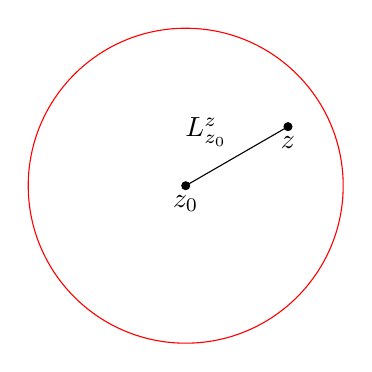
\begin{tikzpicture}[scale = 2]
    \draw [color=red] (0,0) circle (1);
    \draw[fill] (0,0) circle [radius=0.025];
    \node [below] at (0,0) {$z_0$};
    \draw[fill] (30:0.75) circle [radius=0.025];
    \node [below] at (30:0.75) {$z$};
    \draw (0,0) -- (30:0.75);
    \node [above left] at (30:0.75/2) {$L_{z_0}^z$};
\end{tikzpicture}
\end{center}

For all $z\in D$ let:

\begin{align*}
    F(z) = \int_{L_{z_0}^z} f(w) \dif w\\
\end{align*}

This defines a well-defined function $F(z)$ with $F(z_0)=0$. We now will show that $F$ is holomorphic, $C^1$, and an antiderivative of $f$.

Given $z\in D$ and $h$ small s.t. $z+h \in D$, compute:

\begin{align*}
    \frac{F(z+h)-F(z)}{h}=\frac{1}{h} \left( \int_{L_{z_0}^{z+h}} f(w) \dif w - \int_{L_{z_0}^z} f(w) \dif w \right) \\
\end{align*}

Consider the resulting triangle T inscribed in $D_{z_0}$:
\begin{center}
\begin{tikzpicture}[decoration={
    markings,
    mark=at position 0.5 with {\arrow{>}}}
    ]
    \draw [color=red] (0,0) circle (4);
    \draw[fill] (0,0) circle [radius=0.1];
    \node [below left] at (0,0) {$z_0$};
    \draw[fill] (30:3) circle [radius=0.1];
    \node [above right] at (30:3) {$z$};
    \draw[postaction={decorate}]  (0,0) -- (30:3);
    \node [above left] at (30:1.5) {$L_{z_0}^z$};
    
    \draw[postaction={decorate}] (0,0) -- (-15:2.4);
    \draw[fill] (-15:2.4) circle [radius=0.1];
    \node [below] at (-15:2.4) {$z+h$};
    \node [below] at (-15:1.2) {$L_{z_0}^{z+h}$};
    
    \draw[postaction={decorate}] (30:3) -- (-15:2.4);
    \node at (10:3.1) {$L_{z}^{z+h}$};
    \node at (10:1.5) {T};
\end{tikzpicture}
\end{center}

Then note that, by Goursat (integrating in the positive direction):

\begin{align*}
   0 \underset{Gt.}{=}\int_{\partial T} f(w)  \dif w &= \int_{L_{z_0}^{z+h}} f(w)  \dif w + \int_{L_{z+h}^{z}} f(w)  \dif w + \int_{L_{z}^{z_0}} f(w)  \dif w\\
   &= \int_{L_{z_0}^{z+h}} f(w)  \dif w - \int_{L_{z}^{z+h}} f(w)  \dif w - \int_{L_{z_0}^{z}} f(w)  \dif w\\
   &\Downarrow\\
   \frac{1}{h}\left( \int_{L_{z}^{z+h}} f(w)  \dif w \right) &=   \frac{1}{h}\left( \int_{L_{z_0}^{z+h}} f(w)  \dif w - \int_{L_{z_0}^{z}} f(w)  \dif w \right)\\
   &= \frac{F(z+h)-F(z)}{h}
\end{align*}

We then parameterize $L_{z}^{z+h}$ by $z(t) = z+t h, t\in[0,1]$ with $z'(t) = h$:

\begin{align*}
    \frac{F(z+h)-F(z)}{h} &=  \frac{1}{h}\left( \int_0^1 f(z(t)) \cdot z'(t)  \dif t \, \right)\\
    &=\frac{1}{h}\left( \int_0^1 f(z+th) \cdot h \,  \dif t \right)\\
    &= \int_0^1 f(z+th) \,  \dif t\\
    \text{($f \in C^0$; let $h\rightarrow 0$) } &= f(z)
\end{align*}

This proves that F is holomorphic, that F' = f (on D), and that F is $C^1$ (since f is continuous).

\end{proof}

Recall that by the FTC, if f is holomorphic and admits an antiderivative on an open set $\Omega$, then for any closed curve $\gamma$, $\int_\gamma f(z) \dif z = 0$

\begin{corollary}
$\Omega \subset \mathbb{C}$ open, $f:\Omega \rightarrow \mathbb{C}$ holomorphic. Then $\forall D \subset \mathbb{C}$ disc, $\forall \gamma:[a,b] \rightarrow D$ piecewise \textbf{closed} curve:

\begin{align*}
    \int_\gamma f(z) \dif z = 0\\
\end{align*}

\end{corollary}

\begin{proof}
Combine (4.2) and FTC (3.5). Then by (4.2) we find F an antiderivative for f on D. Then by FTC:
\begin{align*}
    \int_\gamma f(z) \dif z = 0\\
\end{align*}
\end{proof}

\begin{remark}
Not every holomorphic function $f:\Omega \rightarrow \mathbb{C}$ has an antiderivative on $\Omega$.

\end{remark}


\begin{example}

$\Omega = \mathbb{C}^* = \mathbb{C} \setminus \{0\}, \, f(z)=\frac{1}{z}$. This function is holomorphic on $\Omega$. 

If there were a function $F:\Omega\rightarrow\mathbb{C}$ holomorphic with $F'(z) = \frac{1}{z}$ (an antiderivative on $\mathbb{C}^*$) then with $\gamma$ being the CCW unit circle:

\begin{align*}
    \int_\gamma f(z) \dif z = 0\\
\end{align*}

But by hand (example not done in the notes) you can calculate that in fact:

\begin{align*}
    \int_\gamma f(z) \dif z = 2\pi i\\
\end{align*}

The mistake is assuming we have an antiderivative on $\mathbb{C}^*$. However by the previous theorem, if we restrict ourselves to any disc $D \subset \mathbb{C}^*$ then $\frac{1}{z}$ does have an antiderivative.

\end{example}

\begin{remark}[Uniqueness of the antiderivative]
If $f:\Omega \rightarrow \mathbb{C}$ holomorphic, and F,G are antiderivatives of f, then $F=G+c $ for some $c\in \mathbb{C}$. Thus the antiderivative is unique up to a constant.
\end{remark}

\begin{proof}
Indeed $(F-G)'= (f-f) = 0$. Thus $F-G$ is holomorphic on $\Omega$ and $F-G$ is constant.
\end{proof}

\begin{remark}[Antiderivative of $\frac{1}{z}$ on D]
Parallel to the real case, an antiderivative of $\frac{1}{z}$ is $log(z)$.
\end{remark}

This will be proved later when we have more powerful tools to work with.

\section{Multivariate Calculus Review}


We present a quick recap of multivariable calculus in $\mathbb{R}^2 = \mathbb{C}$.

Consider $\Omega \subset \mathbb{R}^2 = \mathbb{C}$ open. Consider a countable vector field $\Vec{F}$ on $\Omega$, ie a vector valued function $\Vec{F}:\Omega \rightarrow \mathbb{R}^2$. $\Vec{F}(x,y) = (P(x,y),Q(x,y))$ with $P,Q \in C^1(\overline{\Omega},\mathbb{R})$ (ie P,Q are $C^1$ functions from $\Omega$ to $\mathbb{R}^2$).

If $\gamma$ is a parameterized piecewise smooth curve in $\overline{\Omega}$ then you can define various line integrals:

\begin{align*}
    \int_\gamma P  \dif x , \int_\gamma P  \dif y,\int_\gamma Q  \dif x , \int_\gamma Q  \dif y
\end{align*}

For example if $\gamma(t) = (x(t),y(t)), t\in[a,b]$, then:

\begin{align*}
    \int_\gamma P  \dif x = \int_a^b P(x(t),y(t))\cdot x'(t) \,  \dif t\\
    \int_\gamma P  \dif y = \int_a^b P(x(t),y(t))\cdot y'(t) \,  \dif t\\
\end{align*}

\isubsection{THM: Green's Theorem}

\begin{theorem}[Green's Theorem]
Suppose $\Omega \subset \mathbb{R}^2$ is open and connected, with $\partial \Omega$ given by a piecewise smooth paramterized curve with positive (CCW) orientation. Then given $\Vec{F}(x,y) = (P(x,y),Q(x,y))$ a $C^1$ vector field as above on $\overline{\Omega}$, then:

\begin{align*}
    \int_{\partial \Omega} (P \dif x + Q \dif y) = \int_\Omega \left( \frac{\partial Q}{\partial x} - \frac{\partial P}{\partial y}  \right) \, \underbrace{ \dif A}_{ \dif x \dif y}
\end{align*}
\end{theorem}

\begin{note}
Note that these two notations are the same:

\begin{align*}
    \int_{\partial \Omega} (P \dif x + Q \dif y) &= \oint_{\partial \Omega}\Vec{F}\cdot  \dif \Vec{r}\\
    \text{and } \left( \frac{\partial Q}{\partial x} - \frac{\partial P}{\partial y}  \right) &= \triangledown \times \Vec{F} = curl(\Vec{F})
\end{align*}
\end{note}